\documentclass[12pt,letterpaper]{book}

\usepackage[export]{adjustbox}
\usepackage{amsmath}
\usepackage{amsfonts}
\usepackage{amssymb}
\usepackage[spanish,es-tabla]{babel}
\usepackage{booktabs}
\usepackage{caption}
\usepackage{fancyhdr}
\usepackage{framed}
\usepackage{geometry}
\usepackage{graphicx}
\usepackage[utf8]{inputenc}
\usepackage{listings}
\usepackage{titlesec}
\usepackage{xcolor}
\usepackage{courier}

\usepackage{etoolbox}

\definecolor{light-gray}{HTML}{FFFFFF}
\definecolor{java-comment}{rgb}{0,0.5,0}
\definecolor{java-keyword}{rgb}{0.13,0.13,1}
\definecolor{java-literal}{rgb}{0,0.6,0}
\definecolor{java-annotation}{rgb}{0.46,0.45,0.48}
\definecolor{java-string}{HTML}{B36B00}


%	Cambia los margenes del documento
\geometry{left=23mm,top=20mm,right=23mm}
%	Modifica el formato del comando \section
\titleformat{\section}{\large\bfseries\raggedleft}{Lección \thesection}{1em}{}[{\titlerule[0.8pt]}]
%	Modifica el comando \chapter
\addto\captionsspanish{\renewcommand{\chaptername}{Unidad}}

%	Modifica el encabezado y pie de página
\pagestyle{fancy}
\fancyhf{}
\rhead{\chaptername : Elementos de Interfaces Gráficas}
\lhead{Tópicos Avanzados de Programación}
\rfoot{Página \thepage}
\lfoot{Rafael Rivera López}

%	Agrega espaciado en el interior del las filas de las tablas
\renewcommand{\arraystretch}{1.5}

%Para cambiar el grosor de la línea de encabezado o pie de página
%\renewcommand{\headrulewidth}{2pt}
\renewcommand{\footrulewidth}{0.5pt}

\renewcommand{\lstlistingname}{Código}



\lstset{
  aboveskip=3mm,
  belowskip=3mm,
  literate=
  {á}{{\'a}}1 {é}{{\'e}}1 {í}{{\'i}}1 {ó}{{\'o}}1 {ú}{{\'u}}1
  {Á}{{\'A}}1 {É}{{\'E}}1 {Í}{{\'I}}1 {Ó}{{\'O}}1 {Ú}{{\'U}}1
  {à}{{\`a}}1 {è}{{\`e}}1 {ì}{{\`i}}1 {ò}{{\`o}}1 {ù}{{\`u}}1
  {À}{{\`A}}1 {È}{{\'E}}1 {Ì}{{\`I}}1 {Ò}{{\`O}}1 {Ù}{{\`U}}1
  {ä}{{\"a}}1 {ë}{{\"e}}1 {ï}{{\"i}}1 {ö}{{\"o}}1 {ü}{{\"u}}1
  {Ä}{{\"A}}1 {Ë}{{\"E}}1 {Ï}{{\"I}}1 {Ö}{{\"O}}1 {Ü}{{\"U}}1
  {â}{{\^a}}1 {ê}{{\^e}}1 {î}{{\^i}}1 {ô}{{\^o}}1 {û}{{\^u}}1
  {Â}{{\^A}}1 {Ê}{{\^E}}1 {Î}{{\^I}}1 {Ô}{{\^O}}1 {Û}{{\^U}}1
  {œ}{{\oe}}1 {Œ}{{\OE}}1 {æ}{{\ae}}1 {Æ}{{\AE}}1 {ß}{{\ss}}1
  {ű}{{\H{u}}}1 {Ű}{{\H{U}}}1 {ő}{{\H{o}}}1 {Ő}{{\H{O}}}1
  {ç}{{\c c}}1 {Ç}{{\c C}}1 {ø}{{\o}}1 {å}{{\r a}}1 {Å}{{\r A}}1
  {€}{{\euro}}1 {£}{{\pounds}}1 {«}{{\guillemotleft}}1
  {»}{{\guillemotright}}1 {ñ}{{\~n}}1 {Ñ}{{\~N}}1 {¿}{{?`}}1,
  breaklines=true,
  breakatwhitespace=true,
  postbreak=\raisebox{0ex}[0ex][0ex]{\ensuremath{\color{red}\hookrightarrow\space}},
  language=Java,
  framesep=5pt,
  frame=Trbl,
  basicstyle=\scriptsize\ttfamily,
  columns=fullflexible,
  backgroundcolor=\color{light-gray},
  commentstyle=\color{java-comment},
  keywordstyle=\bfseries\color{java-keyword},
  stringstyle=\color{java-string},
  morecomment=[s][\color{gray}]{@}{\ }
}

\fboxsep=6mm 	%Añade un espacio enter el marco y el contenido de un \fbox{}
\fboxrule=1pt 	%Modifica el grosor del marco de \fbox{}
 
\begin{document}
\chapter{Elementos de Interfaces Gráficas}


\section{Librerías de Interfaz Gráfica}

Java posee varias alternativas para la creación de interfaces gráficas para sus aplicaciones.

\begin{itemize} \itemsep0em
\item [AWT:] El Abstract Window Toolkit es el paquete básico de construcción de interfaces gráficas de Java.
\item [Swing:] Se incluyó dentro de JFC en la versión 1.2 de Java con el objetivo de que los componentes de la interface fueran independientes del sistema operativo en que se ejecutara la aplicación.
\item [Java2D:] Modela primitivas gráficas (líneas, elipses, curvas) en objetos y permite aplicarles transformaciones (rotación, escalado).
\item [Java3D:] Utilizado para crear ambientes y figuras tridimensionales.
\item [JavaFX:] Es la propuesta más reciente que integra varias mejoras al sistema de construcción de interfaces gráficas.
\end{itemize}


\subsection{Componentes Genéricos (AWT)}

AWT es el acrónimo del Abstract Window Toolkit para Java. Se trata de una biblioteca de clases Java para el desarrollo de Interfaces Gráficas de Usuario. La versión original de AWT se desarrolló en sólo dos meses y es la parte más débil de todo lo que representa Java como lenguaje. AWT contiene:

\begin{itemize} \itemsep0em
\item Un gran conjunto de componentes de interfaz de usuario.
\item Un robusto modelo de manejo de eventos.
\item Herramientas gráficas y de imagen, incluyendo forma, color y tipo de letra.
\item Administradores de diseño (layout), para un manejo de ventanas flexible que no dependan de una tamaño o resolución especifico.
\item Clases de transferencia de datos, para copiar y pegar a través del portapapeles de la plataforma en donde se ejecuta la aplicación.
\end{itemize}

\begin{figure}[!htbp]
\begin{framed} \centering
\includegraphics[width=0.8\textwidth]{images/diagrama-clases-awt}
\end{framed}
\caption{Diagrama de clases de los componentes de AWT}
\end{figure} 

\subsection{Componentes Especializados (Swing)}


\begin{itemize} \itemsep0em
\item El paquete Swing es parte de la JFC (Java Foundation Classes) en la plataforma Java.
\item La JFC provee facilidades para ayudar a los desarrolladores a construir interfaces gráficas.
\item Swing abarca componentes como botones, tablas, marcos, etc.
\item Las componentes Swing se identifican porque pertenecen al paquete
\texttt{javax.swing}.
\end{itemize}

Antes de la existencia de Swing, las interfaces gráficas de usuario se construían con AWT (Abstract Window Toolkit), de quien Swing hereda todo el manejo de eventos. Usualmente, para toda componente AWT existe una componente Swing que la reemplaza, por ejemplo, la clase Button de AWT es reemplazada por la clase JButton de Swing (el nombre de todas las componentes Swing comienza con "J").

Las componentes de Swing utilizan la infraestructura de AWT, incluyendo el modelo de eventos AWT, el cual rige cómo una componente reacciona a eventos tales como, eventos de teclado, mouse, etc.

\begin{figure}[!htbp]
\begin{framed} \centering
\includegraphics[width=0.8\textwidth]{images/diagrama-clases-swing}
\end{framed}
\caption{Diagrama de clases de los componentes de SWING}
\end{figure} 

\subsection{Componentes de JavaFX}

JavaFX es el resultado de incorporar aquellos aspectos de provecho de sus predecesores y algunas virtudes de herramientas de GUI de otras tecnologías.

Partiendo del uso de una arquitectura MVC para la construcción de sus componentes gráficos podemos observar el panorama de ventajas que posee. Gracias a esta división entre la lógica y la presentación, se obtiene el benefició de mantenibilidad de las aplicaciones y se agiliza su desarrollo. La unión de la arquitectura MVC, el uso de archivos FXML en la definición de interfaces, la incorporación de hojas de estilo CSS para la personalización de la presentación de los componentes y las APIs para el empleo de archivos multimedia dota al desarrollador con la capacidad de crear interfaces que mejoren la experiencia del usuario.

\begin{figure}[!htbp]
\begin{framed} \centering
\includegraphics[width=0.8\textwidth]{images/diagrama-clases-javafx}
\end{framed}
\caption{Diagrama de clases de los componentes de JavaFX}
\end{figure} 

\begin{figure}[!htbp]
\begin{framed} \centering
\includegraphics[width=0.8\textwidth]{images/diagrama-clases-javafx-controles}
\end{framed}
\caption{Diagrama de clases de algunos controles de JavaFX}
\end{figure} 

\begin{figure}[!htbp]
\begin{framed} \centering
\includegraphics[width=0.8\textwidth]{images/diagrama-clases-javafx-contenedores}
\end{framed}
\caption{Diagrama de clases de los contenedores/administradores de diseño de JavaFX}
\end{figure} 

\subsection{Stage}

La clase Stage modela el contenedor de mayor nivel en las interfaces construidas con JavaFX. Al iniciar una aplicación JavaFX un objeto Stage, comunmente llamado \textit{primaryStage}, es inyectado al método \textit{start} del ciclo de vida de la aplicación, ese objeto será el principal contenedor de la aplicación y en él se mostrará el grafo de escena de la interface.

Adicionalmente se pueden crear más objetos Stage durante la ejecución de la aplicación.

\begin{table} \footnotesize \centering \caption{Métodos comúnes de la clase Stage}
    \label{table:stage-methods}
    \begin{tabular}{l p{11.5cm}} \toprule[1.5pt]
   	\textbf{Método} 			& \textbf{Descripción} \\ \midrule[1.5pt]
   	setScene(Scene value) 		& Añade el grafo de escena al contenedor. \\ \hline
	setTitle(String title)		& Establece el título para mostrar en la barra superior del contenedor. \\ \hline
	show() 						& Vuelve visible para el usuario el contenedor. \\ \hline
	initModality(Modality mod) & Establece la modalidad en que va a funcionar el contenedor. Las modalidades son: \verb|Modality.NONE|, \verb|Modality.WINDOW_MODAL|, \verb|Modality.APPLICATION_MODAL|.  \\ \bottomrule[1.5pt]
    \end{tabular}
\end{table}


\subsection{Scene}

El Scene Graph o grafo de escena es una representación jerárquica de la
interface de usuario de la aplicación. Para cada ventana que tenga la aplicación existirá un grafo de escena asociado a ella. El grafo contiene nodos que son todos los elementos visuales de la interface: controles, primitivas gráficas, layouts, imágenes, etc.

Cada nodo tiene una clase asociada a su estilo y un identificador único. Todos los nodos, con excepción de la raíz, poseen un padre y cero o más nodos hijos. Usar este tipo de representación tiene dos ventajas: la primera es que se pueden aplicar efectos, transformaciones y escuchadores de eventos a nodos particulares o a un sub-árbol de nodos del grafo a la vez; la segunda es que se mejora el desempeño de la aplicación usando estrategias de optimización de renderizado de la escena.

\subsection{Paneles y Administradores de Diseño}

Los paneles son contenedores que agrupan a otros componentes. Anteriormente, con Swing, los conceptos de contenedor y administrador de diseño eran independientes, ahora con JavaFX ambos conceptos están tan ligados al grado que las clases contenedoras ya tienen un administrador de diseño establecido que no puede ser cambiado.

Como ya se explicó en el tema Elementos de una interfaz Gráfica, la importancia de los administradores de diseño reside, principalmente, en la capacidad para ubicar los componentes gráficos de la interface siguiendo un patrón de distribución y ubicación. JavaFX ofrece 9 administradores de diseño distintos, suficientes para la mayoría de los casos. Las clases están contenidas en el paquete \texttt{javafx.scene.layout}.

A continuación, la tabla \ref{table:layouts}, describe brevemente cada administrador de diseño.
%Comentar el administrador de diseño que se usa por defecto y describir los admnistradores de diseño más importantes.
\begin{table} \footnotesize \centering \caption{Administradores de diseño en JavaFX} \label{table:layouts}
    \begin{tabular}{l p{14cm}} \toprule[1.5pt]
   	\textbf{Layout} 	& \textbf{Descripción} \\ \midrule[1.5pt]
   	AnchorPane 			& Coloca los componentes en una posición relativa al los bordes del contenedor. \\ \hline
   	BorderPane 			& Divide el admnistrador de diseño en 5 secciones: norte, sur, este, oeste y centro. \\ \hline
	FlowPane 			& Ubica los componentes que contiene en posición superior izquierda, uno después de otro conforme estos fueron añadidos. Ajusta el tamaño de sus componentes al mínimo. \\ \hline
	GridPane 			& Divide el contenedor en filas y columnas permitiendo ubicar los controles en celdas específicas.\\ \hline
	HBox 				& Coloca los controles siguiendo un acomodo horizontal ordenando de izquierda a derecha.\\ \hline
	Pane 				& Clase base de la que derivan el resto de administradores de diseño. Útil cuando se ubican los componentes de la interfaz mediante posición absoluta.\\ \hline
	StackPane 			& Ubica los componentes gŕaficos al centro del panel apilandolos uno encima de otro acorde al orden en que fueron añadidos. \\ \hline
	TilePane 			& Ubica los componentes en una malla horizontal o vertical cuyas celdas poseen el el mismo espacio disponible respecto al tamaño mínimo preferido del componente más grande contenido.\\ \hline
	VBox 				& Coloca los controles verticalmente ordenando de arriba hacia abajo.\\ \bottomrule[1.5pt]
    \end{tabular}
\end{table}

\begin{minipage}[c]{0.95\textwidth}
\lstinputlisting[
	caption=Aplicación de demostración con componentes y administrador de diseño sencillo., 
	label=code:components1
]{source-codes/t-1-2-components-1.java}
\end{minipage}

\begin{minipage}[c]{0.95\textwidth}
\lstinputlisting[
	caption=Clase auxiliar para definir la interfaz de usuario.,
	label=code:components2
]{source-codes/t-1-2-components-2.java}
\end{minipage}

\begin{figure}[!htbp] \centering \fboxsep=1mm
\fbox{\includegraphics[width=0.8\textwidth]{images/app-ejemplo-controles}}
\caption{Aplicación producida los códigos \ref{code:components1} y \ref{code:components2}}
\end{figure} 

\newpage
\subsection{Menús}

En JavaFX los menús pueden añadirse a cualquier administrador de diseños a diferencia de Swing donde solo se podían añadir a instancias de JFrame. Se requieren tres clases para hacer uso de menús en una interfaz gráfica.

\begin{itemize} \itemsep0em 
\item \textbf{MenuBar:} Define la barra de menú para la ventana.
\item \textbf{Menu:} Define el menú incluido en la barra menú.
\item \textbf{MenuItem:} Define la opción de un menú.
\end{itemize}

\begin{table} \footnotesize \centering \caption{Métodos asociados al manejo de menús}    
    \begin{tabular}{l p{14cm}} \toprule[1.5pt]
   	\textbf{Método} 	& \textbf{Descripción} \\ \midrule[1.5pt]
   	getMenus() 			& Método de la clase MenuBar que devuelve la lista de menús asociados a la barra de menú. \\ \hline
	getItems()			& Método de la clase Menu que devuelve la lista de elementos de menú asociados. \\ \toprule[1.5pt]
    \end{tabular}
\end{table}

% Ejemplo básico mostrando la construcción de una barra de menú.
% Ejemplo avanzado mostrando la construcción de una barra de menú utilizando
% imagenes y acciones vinculadas al teclado.

\begin{figure}[!htbp]
\begin{framed} \centering
\includegraphics[width=0.7\textwidth]{images/diagrama-clases-menu}
\end{framed}
\caption{Diagrama de clases de los componentes de tipo Menu}
\end{figure} 

\begin{minipage}[c]{0.95\textwidth}
\lstinputlisting[
	caption=Aplicación de demostración con componentes de tipo menú.,
	label=code:menu1
]{source-codes/t-1-2-menu-1.java}
\end{minipage}

\begin{minipage}[c]{0.95\textwidth}
\lstinputlisting[
	caption=Clase auxiliar para construir la barra de menú de la aplicación.,
	label=code:menu2
]{source-codes/t-1-2-menu-2.java}
\end{minipage}

\begin{figure}[!h] \centering \fboxsep=1mm
\fbox{\includegraphics[width=0.8\textwidth]{images/ejemplo-menus-1}}
\caption{Aplicación producida con los códigos \ref{code:menu1} y \ref{code:menu2}}
\end{figure} 

Utilizando el código \ref{code:menu1} junto al código \ref{code:menu3} se obtiene una aplicación que ejemplifica el uso de carácteres mnemónicos para identificar los menús al presionar la tecla \texttt{ALT} y el uso de combinaciones de teclas para seleccionar un item de menú sin la necesidad de interactuar directamente con la interface. 

\begin{table} \footnotesize \centering \caption{Métodos de utilidad de MenuItem}
    \begin{tabular}{l p{11cm}} \toprule[1.5pt]
   	\textbf{Método} 								& \textbf{Descripción} \\ \midrule[1.5pt]
   	{\scriptsize setMnemonicParsing(boolean b)} 	& Si la propiedad mnemonicParsing es establecida como \texttt{true} se hará un parseo del texto del MenuItem en busca del carácter \verb|_|, al ser hallado se establecerá el carácter que le suceda como mnemónico. \\ \hline
   	{\scriptsize setAccelerator(KeyCombination k)} & Define la combinación de teclas que ejecutarán la acción asociada a un MenuItem. \\ \hline
	setGraphic(Node g) 								& Establece un componente gráfico para mostrar con junto al MenuItem. \\ \bottomrule[1.5pt]
    \end{tabular}
\end{table}

\textbf{KeyCombination}\\
Como su nombre lo indica, KeyCombination representa una combinación de teclas que puede asociarse a una opción de menú para ejecutar su acción. Se tienen dos alternativas para la creación de instancias de KeyCombination: con alguno de sus dos constructores y con un método estático \texttt{\textit{keyCombination(String s)}}.

\begin{minipage}[c]{0.95\textwidth}
\lstinputlisting[
	caption=Aplicación de demostración con acciones en menús e imágenes.,
	label=code:menu3
]{source-codes/t-1-2-menu-3.java}
\end{minipage}

\begin{figure}[!hbp] \centering \fboxsep=1mm
\fbox{\includegraphics[width=0.7\textwidth]{images/app-ejemplo-menus-2}}
\caption{Aplicación producida con los códigos \ref{code:menu1} y \ref{code:menu3}}
\end{figure} 

\newpage
\subsection{TabPane}

TabPane es un control de interfaz gráfica, no un administador de diseño como se podría pensar. La ventaja de este control es que funciona como un contenedor en el que se pueden organizar secciones de la interface en pestañas.

Estas son algunas características de TabPane:

\begin{itemize} \itemsep0em
\item Solamente es visible el contenido de una de las pestañas a la vez.
\item Las pestañas pueden incluir texto y/o un ícono.
\item La ubicación de las pestañas puede ser en la parte superior, inferior, derecha o izquierda del contenedor.
\end{itemize}

\begin{table}[!hbtp] \footnotesize \centering \caption{Recursos útiles para el uso de TabPane} \label{table:layouts}
    \begin{tabular}{p{3.8cm} p{0.1cm} p{12cm}} \toprule[1.5pt]
   	\textbf{Clase, Constructor o Método} 	& & \textbf{Descripción} \\ \midrule[1.5pt]
	javafx.scene.control.Tab				& & Clase modelo de las pestañas. \\ \hline
   	TabPane(Tab... tabs)    				& & Construye un nuevo TabPane con las pestañas especificadas en el constructor. \\ \hline
   	getTabs() 								& & Devuelve la lista de pestañas del contenedor, a esa lista se pueden añadir o quitar Tabs. \\ \hline
	setSide(Side s) 						& & Define la ubicación de las pestañas. \\ \bottomrule[1.5pt]
    \end{tabular}
\end{table}

Los códigos \ref{code:tab-1}, \ref{code:tab-2} y \ref{code:tab-3} ejemplifican una aplicación que utiliza el control TabPane. Como extra también se demuestran las capacidades programáticas para configurar apariencia, ubicación, tamaño y tamaño referente al contenedor de los componentes.

\begin{minipage}[c]{0.95\textwidth}
\lstinputlisting[
	caption=Aplicación de demostración del uso de TabPane.,
	label=code:tab-1
]{source-codes/t-1-2-tab-1.java}
\end{minipage}

\begin{minipage}[c]{0.95\textwidth}
\lstinputlisting[
	caption=Subclase de TabPane para la demostración (Parte 1).,
	label=code:tab-2
]{source-codes/t-1-2-tab-2-p1.java}
\end{minipage}

\begin{minipage}[c]{0.95\textwidth}
\lstinputlisting[
	caption=Subclase de TabPane para la demostración (Parte 2).,
	label=code:tab-3
]{source-codes/t-1-2-tab-2-p2.java}
\end{minipage}

\begin{figure}[!htbp] \centering \fboxsep=1mm
\fbox{\includegraphics[width=0.9\textwidth]{images/app-code-4}}
\caption{Aplicación creada con los códigos \ref{code:tab-1}, \ref{code:tab-2} y \ref{code:tab-3}}.
\end{figure} 

\newpage
\subsection{Dialog: Alert, TextInputDialog y ChoiceDialog}

JavaFX provee estas tres clases para mostrar mensajes, pedir un dato o solicitar la selección de una opción al usuario mediante una ventana emergente. La mayoría de los casos en que se pueda necesitar la interacción con el usuario mediante ventanas emergentes se pueden cubrir con estas clases.

Algunas características de las ventanas emergentes son las siguientes:

\begin{itemize} \itemsep0em
\item Su comportamiento puede ser modal o bloqueante. El comportamiento modal permite al usuario seguir interactuando con la interface de la aplicación mientras que el bloqueante impide cualquier acción que no sea dentro de la ventana emergente.

\item Las ventanas emergentes están vinculadas a la ventana principal de la aplicación, si esta se cierra, maximiza o minimiza las ventanas emergentes ejecurarán el mismo comportamiento.

\item Son subclases de \texttt{javafx.scene.control.Dialog}. 
\end{itemize}

\begin{table} \footnotesize \centering \caption{Métodos de utilidad de la clase Dialog}
    \begin{tabular}{p{4cm} p{12cm}} \toprule[1.5pt]
   	\textbf{Método} 			& \textbf{Descripción} \\ \midrule[1.5pt]
   	setTitle(String t)			& Define el título que se mostrará en el marco. 	\\ \hline
   	setHeaderText(String t) 	& Define el texto de la cabecera del mensaje. 		\\ \hline
   	setContentText(String t) 	& Define el mensaje de la ventana emergente. 		\\ \hline
   	{\scriptsize setAlertType(AlertType t)} & Establece el tipo de la ventana emergente (En el caso de \texttt{Alert}). Los tipos disponibles son \texttt{NONE}, \texttt{CONFIRMATION}, \texttt{INFORMATION}, \texttt{WARNING}, \texttt{ERROR}. 	\\ \hline
   	show() 						& Muestra la ventana emergente en modo modal (no espera por la interacción del usuario). \\ \hline
   	showAndWait() 				& Muestra la ventana emergente en modo bloqueante (espera por la interacción del usuario). \\ \bottomrule[1.5pt]
    \end{tabular}
\end{table}

\begin{figure}[!htbp] \centering \fboxsep=1mm
\fbox{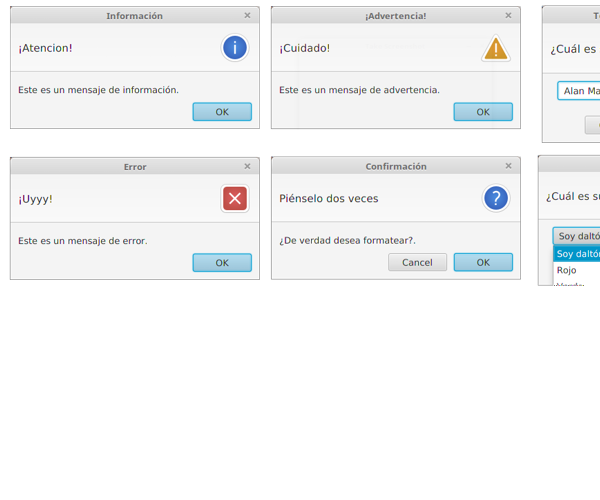
\includegraphics[width=0.9\textwidth]{images/dialogs}}
\caption{Diálogos de ejemplo}
\end{figure} 

\subsection{FileChooser}

Permite navegar por el sistema de archivos de la plataforma donde se ejecuta la aplicación y su look and feel (apariencia) es dependiente del sistema operativo. A diferencia de otros controles de interface, la clase \texttt{FileChooser} pertenece al paquete \texttt{javafx.scene}.

Estos son algunos métodos importantes de esta clase.

\begin{table} \footnotesize \centering \caption{Métodos de utilidad de la clase Dialog}
    \begin{tabular}{p{5cm}  p{11cm}} \toprule[1.5pt]
   	\textbf{Método} & \textbf{Descripción} \\ \midrule[1.5pt]
   	showOpenDialog(Window w)	
   	& Permite seleccionar \textbf{un} archivo mediante el dialogo de navegación del sistema de archivos. Devuelve una instancia de la clase File o null si no se seleccionó un archivo. El parámetro \texttt{w} debe ser la ventana a la que estará vinculada la ventana de navegación. \\ \hline
   	{\scriptsize showOpenMultipleDialog(Window w)} 
   	& Permite seleccionar \textbf{multiples} archivos mediante el dialogo de navegación del sistema de archivos. Devuelve una instancia de la clase File o null si no se seleccionó un archivo. El parámetro \texttt{w} debe ser la ventana a la que estará vinculada la ventana de navegación. \\ \hline
   	showSaveDialog(Window w)
   	& Permite guardar un archivo mediante el dialogo de navegación del sistema de archivos. Devuelve una instancia de la clase File o null si no se seleccionó un archivo. El parámetro \texttt{w} debe ser la ventana a la que estará vinculada la ventana de navegación. \\ \hline
   	getExtensionFilters() & Devuelte la lista de filtros de archivos por extensión, a esa lista se pueden añadir o quitar filtros. \\ \bottomrule[1.5pt]
    \end{tabular}
\end{table}

\begin{figure}[!htbp] \centering \fboxsep=1mm
\fbox{\includegraphics[width=0.9\textwidth]{images/app-code-6}}
\caption{Diálogo de navegación por el sistema de archivos}
\end{figure} 


% Explicación del componente/control para seleccionar archivos del disco duro.
% Mostrar sus métodos más utilizados.

\subsection{ColorPicker}

Este control posibilita la selección de un color. Su comportamiento consiste en mostrar una paleta de colores predefinidos al usuario, una vez que el usuario hace su elección la paleta se oculta y se puede obtener el color seleccionado. También puede mostrar una ventana emergente para que el usuario cree un color a sus necesidades.

\begin{figure}[!htbp] \centering \fboxsep=1mm
\fbox{\includegraphics[width=0.9\textwidth]{images/app-code-7}}
\caption{Ventana emergente para selección de colores}
\end{figure} 

% Explicación del componente/control para seleccionar archivos del disco duro.
% Mostrar sus métodos más utilizados.

\subsection{ScrollPane}
% Explicación del componente/control para desplazar el contenido visible.
% Mostrar sus métodos más utilizados.
Al igual que TabPane, ScrollPane es un control y no un panel, y ofrece un área desplazable de visualización de su contenido.

\begin{table} \footnotesize \centering \caption{Métodos de utilidad de la clase ScrollPane}
    \begin{tabular}{p{5.5cm} p{10.5cm}} \toprule[1.5pt]
   	\textbf{Método} & \textbf{Descripción} \\ \midrule[1.5pt]   	
	setHbarPolicy(ScrollBarPolicy p)	& Define el comportamiento para mostrar las barra de desplazamiento horizontal. Los valores posibles son \verb|ScrollBarPolicy.ALWAYS}|, \verb|ScrollBarPolicy.AS_NEEDED}|, \verb|ScrollBarPolicy.NEVER|. \\ \hline
	setVbarPolicy(ScrollBarPolicy p)	& Define el comportamiento para mostrar las barras de desplazamiento vertical. Los valores posibles son \verb|ScrollBarPolicy.ALWAYS}|, \verb|ScrollBarPolicy.AS_NEEDED}|, \verb|ScrollBarPolicy.NEVER|. \\ \bottomrule[1.5pt]
    \end{tabular}
\end{table}

\begin{figure}[!htbp] \centering \fboxsep=1mm
\fbox{\includegraphics[width=0.5\textwidth]{images/app-code-8}}
\caption{Ejemplo de una instancia de ScrollPane que contiene una imagen}
\end{figure} 

\subsection{SplitPane}
% Explicación del componente/control SplitPane que permite manipular el espacio que destina a los componentes que contiene.
% Mostrar sus métodos más utilizados.

Este control puede contener dos o más secciones acomodadas vertical u horizontalmente, separando las secciones con divisores que pueden ser arrastrados para dar más espacio a una de las secciones.

\begin{figure}[!htbp] \centering \fboxsep=1mm
\fbox{\includegraphics[width=0.5\textwidth]{images/app-code-9}}
\caption{Ejemplo del uso de SplitPane que contiene tres paneles distintos}
\end{figure}

\subsection{ToolBar}

% Explicación del componente/control ToolBar que permite concentrar componentes en un área para su acceso rápido.
% Mostrar sus métodos más utilizados.

Las barras de herramientas facilitan al usuario el acceso a aquellas funciones que se utilizan con mayor frecuencia en las aplicaciones. Para tal propósito JavaFX tiene el control ToolBar al que se pueden añadir instancias de cualquier subclase de \texttt{Node}.	

\begin{figure}[!htbp] \centering \fboxsep=1mm
\fbox{\includegraphics[width=0.8\textwidth]{images/app-code-10}}
\caption{Ejemplo del uso de ToolBar con orientación vertical}
\end{figure}


\subsection{Apariencia de la Aplicación}

%Mencionar las alternativas para personalizar la apareicencia de los componentes gráficos.

Con JavaFX la presentación visual de los controles de la interface es muy personalizable gracias a las reglas CSS. Se tienen dos alternativas para modificar la apariencia de los controles, la primera es mediante una modificación programática de las propiedades visuales de los controles a través del métodos heredados por la clase \texttt{javafx.scene.Node} y la interfaz \texttt{javafx.css.Styleable}; la segunda alternativa la asociación de clases CSS mediante el atributo \texttt{class} de los elementos ligados a los controles en la definición de interfaces mediante archivos FXML. Detalles de la segunda alternativa se explican en la sección \textsl{Scene Builder}.

\begin{table} \footnotesize \centering \caption{Métodos útiles para la personalización de la apariencia de controles}
    \begin{tabular}{l l p{9cm}} \toprule[1.5pt]
   	\textbf{Método} 	& \textbf{Clase}					& \textbf{Descripción} \\ \midrule[1.5pt]
   	setStyle(String s)	& \texttt{javafx.scene.Node}		& Modifica la propiedad visual del control, su sintaxis es \texttt{ ``propiedad : valor'' }. \\ \hline
   	getStylesheets()	& \texttt{javafx.scene.Parent} 	& Devuelte la lista URLs de \textbf{archivos} CSS asociados al nodo, a esa lista se pueden añadir o quitar URLs. \\ \hline
	getStyleClass()		& \texttt{javafx.css.Styleable} 	& Devuelve la lista de clases asociadas al control, a esa lista se pueden añadir o quitar clases CSS. \\ \bottomrule[1.5pt]   
    \end{tabular}    
\end{table}

\subsection{Scene Builder} \label{subsec:scene-builder}

% Exposición del propósito de la herramienta.
% Explicación de los componentes y áreas de la herramienta.
% Mostrar sus métodos más utilizados.

Una de las mejoras más sobresalientes incluidas en JavaFX es el diseño de interfaces gráficas mediante el lenguaje de marcado FXML, manera similar en la que se construyen interfaces en los estándares web mediante HTML. FXML es un lenguaje derivado de XML y significa \texttt{F}x e\texttt{X}tensible \texttt{M}arkup \texttt{L}anguage, fue incluido en el conjunto de tecnologías que acompañan a JavaFX desde su versión 2.0.

Para facilitar la actividad de construcción de interfaces Oracle lanzó Scene Builder, una herramienta de diseño mediante un editor gráfico. Actualmente Oracle sólo proporciona Scene Builder como código fuente mediante el proyecto OpenJFX. Sin embargo, la empresa Gluon dedicada a la creación de soluciones y herramientas basadas en Java, mantiene soporte a una versión  de Scene Builder. Scene Builder de Gluon\footnote{http://gluonhq.com/products/scene-builder/} puede ser utilizado como una aplicacion independente o integrarse como plugin a los entornos de desarrollo NetBeans, Eclipse e IntelliJ.

\begin{figure}[!htbp] \centering \fboxsep=1mm
\fbox{\includegraphics[width=0.95\textwidth]{images/scene-builder-gluon-arrows}}
\caption{Interfaz de Scene Builder 2.0}
\end{figure}

\newpage

\subsection{Ejemplo de una aplicación de chat}

La figura \ref{fig:chat} muestra una interface para un chat creado con Scene Builder.

\begin{figure}[!htbp] \centering \fboxsep=1mm
\fbox{\includegraphics[width=0.7\textwidth]{images/chat}}
\caption{Captura de pantalla a la interfaz del chat}
\label{fig:chat}
\end{figure} 

\begin{minipage}[c]{0.95\textwidth}
\lstinputlisting[
	caption=Clase principal donde se carga el archivo FXML.,
	label=code:chat-layout
]{source-codes/t-1-2-chat1.java}
\end{minipage}

\begin{minipage}[c]{0.95\textwidth}
\lstinputlisting[
	caption		= Archivo FXML creado Scene Builder para la interface del chat.,
	label		= code:chat-layout,
	language 	= xml
]{source-codes/t-1-2-chat2.fxml}
\end{minipage}



\end{document}